% Author: Izaak Neutelings (September 2021)
% Inspiration:
%   https://www.asimovinstitute.org/neural-network-zoo/
%   https://www.youtube.com/watch?v=aircAruvnKk&list=PLZHQObOWTQDNU6R1_67000Dx_ZCJB-3pi&index=1
\documentclass[border=3pt,tikz]{standalone}
\usepackage{amsmath} % for aligned
\usepackage{listofitems} % for \readlist to create arrays
\usetikzlibrary{arrows.meta} % for arrow size
\usepackage[outline]{contour} % glow around text
\contourlength{1.4pt}
\pdfminorversion=5

% COLORS
\usepackage{xcolor}
\colorlet{myred}{red!80!black}
\colorlet{myblue}{blue!80!black}
\colorlet{mygreen}{green!60!black}
\colorlet{myorange}{orange!70!red!60!black}
\colorlet{mydarkred}{red!30!black}
\colorlet{mydarkblue}{blue!40!black}
\colorlet{mydarkgreen}{green!30!black}

% STYLES
\tikzset{
  >=latex, % for default LaTeX arrow head
  node/.style={thick,circle,draw=myblue,minimum size=22,inner sep=0.5,outer sep=0.6},
  node in/.style={node,green!20!black,draw=mygreen!30!black,fill=mygreen!25},
  node hidden/.style={node,blue!20!black,draw=myblue!30!black,fill=myblue!20},
  node convol/.style={node,orange!20!black,draw=myorange!30!black,fill=myorange!20},
  node out/.style={node,red!20!black,draw=myred!30!black,fill=myred!20},
  connect/.style={thick,mydarkblue}, %,line cap=round
  connect arrow/.style={-{Latex[length=4,width=3.5]},thick,mydarkblue,shorten <=0.5,shorten >=1},
  node 1/.style={node in}, % node styles, numbered for easy mapping with \nstyle
  node 2/.style={node hidden},
  node 3/.style={node out}
}
\def\nstyle{int(\lay<\Nnodlen?min(2,\lay):3)} % map layer number onto 1, 2, or 3

\begin{document}

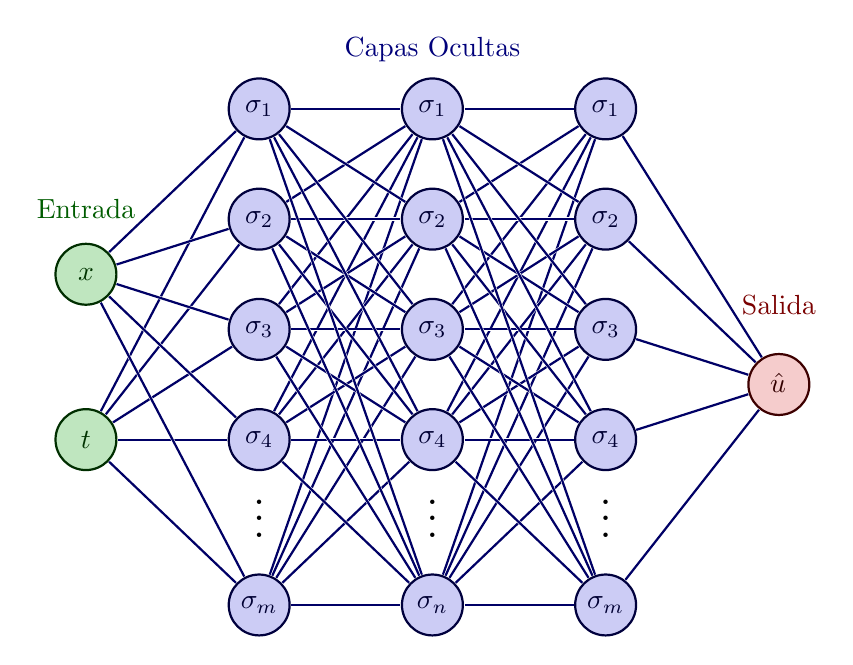
\begin{tikzpicture}[x=2.2cm,y=1.4cm]
    \message{^^JNeural network, shifted}
    \readlist\Nnod{2,5,5,5,1} % array of number of nodes per layer
    \readlist\Nstr{n,m,n,m,} % array of string number of nodes per layer
    \readlist\Cstr{\strut x,\sigma,\sigma,\sigma,\hat{u}} % array of coefficient symbol per layer
    \def\yshift{0.5} % shift last node for dots
    
    \message{^^J  Layer}
    \foreachitem \N \in \Nnod{ % loop over layers
      \def\lay{\Ncnt} % alias of index of current layer
      \pgfmathsetmacro\prev{int(\Ncnt-1)} % number of previous layer
      \message{\lay,}
      \foreach \i [evaluate={\c=int(\i==\N); \y=\N/2-\i-\c*\yshift;
                   \index=(\i<\N?int(\i):"\Nstr[\lay]");
                   \x=\lay; \n=\nstyle; \luis=int(\i) }] in {1,...,\N}{ % loop over nodes
        
        \ifnum\lay=1
            \ifnum\luis=1
                \node[node \n] (N\lay-\luis) at (\x,\y) {$x$};
            \else
                \node[node 1] (N\lay-\luis) at (\x,\y) {$t$};
            \fi
        \else   
            \node[node \n] (N\lay-\i) at (\x,\y) {$\Cstr[\lay]_{\index}$};
        \fi
  
        % CONNECTIONS
        \ifnum\lay>1 % connect to previous layer
          \foreach \j in {1,...,\Nnod[\prev]}{ % loop over nodes in previous layer
            \draw[connect,white,line width=1.2] (N\prev-\j) -- (N\lay-\i);
            \draw[connect] (N\prev-\j) -- (N\lay-\i);
            %\draw[connect] (N\prev-\j.0) -- (N\lay-\i.180); % connect to left
          }
        \fi % else: nothing to connect first layer
        
      }
      \ifnum\N>2
       \path (N\lay-\N) --++ (0,1+\yshift) node[midway,scale=1.5] {$\vdots$};
      \fi
    }
  
  
  % LABELS
  \node[above=5,align=center,mygreen!60!black] at (N1-1.90) {Entrada};
  \node[above=2,align=center,myblue!60!black] at (N3-1.90) {Capas Ocultas};
  \node[above=10,align=center,myred!60!black] at (N\Nnodlen-1.90) {Salida};
  
\end{tikzpicture}


\end{document}